\documentclass{article}
\usepackage{amsmath}
\usepackage[mathletters]{ucs}
\usepackage[utf8x]{inputenc}
\usepackage[margin=1.5in]{geometry}
\usepackage{enumerate}
\newtheorem{theorem}{Theorem}
\usepackage[dvipsnames]{xcolor}
\usepackage{pgfplots}
\pgfplotsset{compat/show suggested version=false}
\setlength{\parindent}{0cm}
\usepackage{graphics}
\usepackage{graphicx} % Required for including images
\usepackage{subcaption}
\usepackage{bigintcalc}
\usepackage{pythonhighlight} %for pythonkode \begin{python}   \end{python}
\usepackage{appendix}
\usepackage{arydshln}
\usepackage{physics}
\usepackage{tikz-cd}
\usepackage{booktabs} 
\usepackage{adjustbox}
\usepackage{mdframed}
\usepackage{relsize}
\usepackage{physics}
\usepackage[thinc]{esdiff}
\usepackage{fixltx2e}
\usepackage{esint}  %for lukket-linje-integral
\usepackage{xfrac} %for sfrac
\usepackage{hyperref} %for linker, må ha med hypersetup
\usepackage[noabbrev, nameinlink]{cleveref} % to be loaded after hyperref
\usepackage{amssymb} %\mathbb{R} for reelle tall, \mathcal{B} for "matte"-font
\usepackage{listings} %for kode/lstlisting
\usepackage{verbatim}
\usepackage{graphicx,wrapfig,lipsum,caption} %for wrapping av bilder
\usepackage{mathtools} %for \abs{x}
\usepackage[norsk]{babel}
\definecolor{codegreen}{rgb}{0,0.6,0}
\definecolor{codegray}{rgb}{0.5,0.5,0.5}
\definecolor{codepurple}{rgb}{0.58,0,0.82}
\definecolor{backcolour}{rgb}{0.95,0.95,0.92}
\pagecolor[rgb]{0.075,0.075,0.075} \color[rgb]{1,1,1}

\lstdefinestyle{mystyle}{
    backgroundcolor=\color{backcolour},   
    commentstyle=\color{codegreen},
    keywordstyle=\color{magenta},
    numberstyle=\tiny\color{codegray},
    stringstyle=\color{codepurple},
    basicstyle=\ttfamily\footnotesize,
    breakatwhitespace=false,         
    breaklines=true,                 
    captionpos=b,                    
    keepspaces=true,                 
    numbers=left,                    
    numbersep=5pt,                  
    showspaces=false,                
    showstringspaces=false,
    showtabs=false,                  
    tabsize=2
}

\lstset{style=mystyle}
\author{Oskar Idland}
\title{Oscillations and Waves}
\date{}
\begin{document}
\maketitle
\newpage
\begin{figure}[h!]
  \centering
  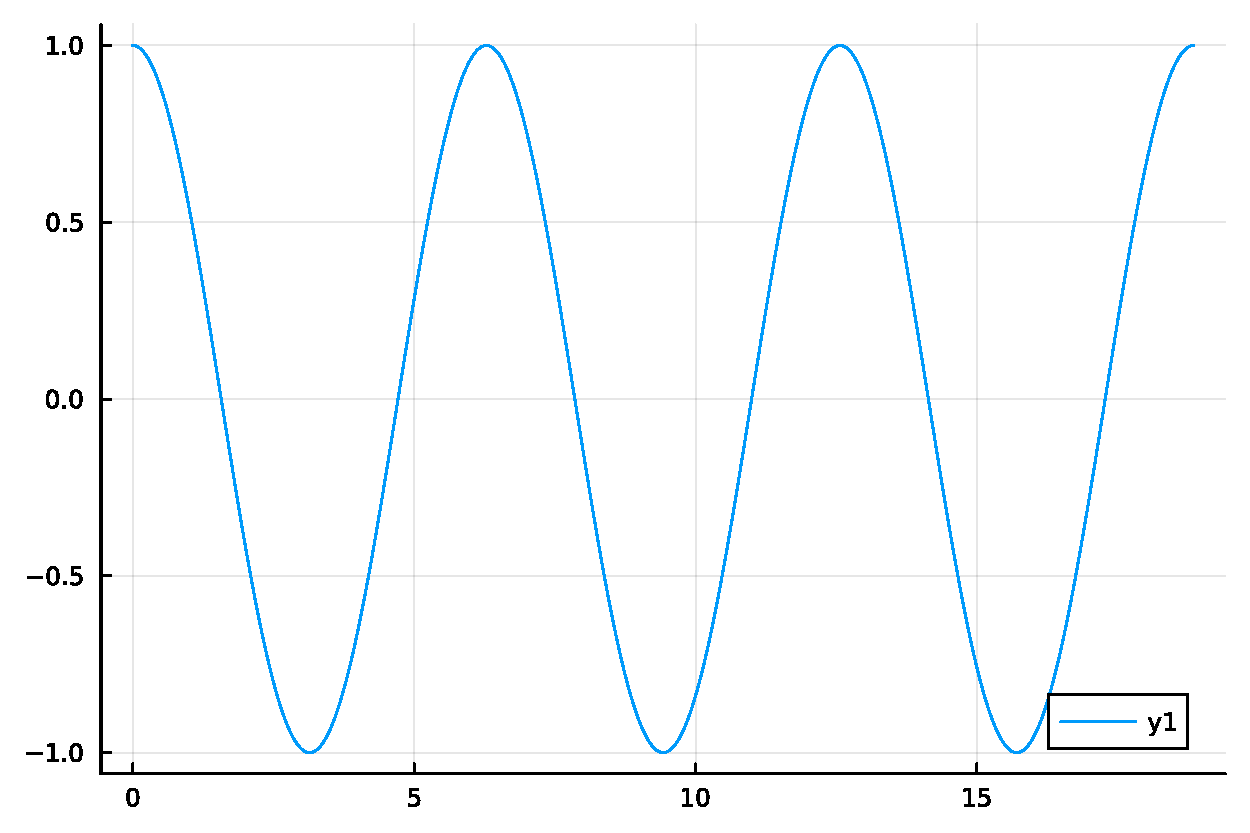
\includegraphics[scale = .5]{Figures/cosine_curve.pdf}
  \caption{Cosinus bølge}
  \label{fig: cosine_curve}
\end{figure}
Vi kan beskrive en svingning på flere måter.

\begin{enumerate}[I]
\item  $x(t) = A \cos (ωt + ϕ)$
\item  $x(t) = A\cos (ωt) + B \sin (ωt)$
\item  $e^{iωt} = \cos (ωt) + i \sin (ωt)$
\end{enumerate}


\[
x(t) = A \cos (\frac{2π}{T}t), f = \frac{1}{T}
\]
A er amplituden og $f$ er frekvensen til svingningen og måles i Hz. 
\[
x(t) = \cos (\underbrace{2πf}_{\omega} ⋅ t )
\]
Hvor $ω$ er vinkelfrekvensen og måles i rad/s.
        
\subsubsection*{I}
\[
x(t) = A \cos (ωt + ϕ)
\]
Hvor $ϕ$ er faseforskyvningen til svingningen. Vi kan også konvertere cosinus til sinus ved å legge til 90 grader 
\[
x(t) = A \sin (ωt + ϕ + \frac{π}{2}).
\]

\subsubsection*{II}
  
En annen måte å beskrive bølgen på kan være følgende
\[
x(t) = A\cos (ωt) + B \sin (ωt)
\]

\subsubsection*{III}
\[
e^{iωt} = \cos (ωt) + i \sin (ωt)
\]



\end{document}